
\chapter{Methods and Results}
\label{methods} % Always give a unique label
%use \chaptermark{}
% to alter or adjust the chapter heading in the running head

This chapter introduces methods and methodology of this work.

\section{System Architecture}
\label{sec:sysArch}
System architecture is shown on figure .. Include block diagram

\section{Sensor Placement Optimization}
\label{sec:SimMod}

	Sensor location on sleeves, shaft and cannula - include COMSOL studies
	Strain Gauge Placement
	A qualitative analysis was done in Solidworks to assess better placement of the strain gauges on the shaft or cannula. First we found elasticity modulus of the shaft and cannula, and used them for further analysis.
	The shaft and cannula material are unknown, so we studied their elasticity modulus, .. experimentally.

	\subsection{Elasticity Modulus Measurements}
	\label{sec:ElasMod}
	Elasticity Modulus of the shaft and the cannula were found experimentally (Figure 1). One end of the observing sample (shaft or cannula) was fixed and the force was applied on the other end. We used weights: 250g for the shaft and 555g for the cannula. The deformation was detected with dial indicator XXX. Experiment was done 5 times, average displacement value was used.
	...
	\subsection{Density Measurements}
	\label{sec:DenMeas}

\section{Requirements for the Device}
	\label{sec:DevReq}
	From the literature review, following requiremetns for the device were developed:
	Biocompatibility
	
	Linearity
	
	Range of forces 
	Highest gripping force in Da Vinci tool was seen in the Hemo-lok[R] clip applier (39.92 [+ or -] 0.89 N).
	0.3 - 11 N. 
	Tensile strength and failure load of sutures for robotic surgery
	Others

\section{Mechanical Design}
\label{sec:mechDes}

	\subsection{Strain Gauge}
	\label{sec:SGReq}
	According to the manual for strain gauge selection provided by Vishay Micro-Measurements. The strain gauge should have following parameters:
	• Gauge length is 0.8 mm. Ideally gauge length should be 10 \% of the shaft radius;
	• Single grid;
	• Isoelastic (D alloy) that has higher gauge factor with E backing;
	• Encapsulated with pre attached leads;
	• Resistance – 120 Ohms;
	• Gauge factor - 2;
	• STC – number (self-temperature-compensation): DY – dynamic
	Since the diameter of the shaft is only 8.5 mm, one of the most important parameters, in this
	case, is the size of the strain gauge. Another important parameter is gauge‘s resistance, sensitivity
	of the strain gauge drastically depends on this parameter. Strain gauges with different resistivity
	were used (350 and 120 Ohms and sizes of 6 x 2.5 mm).

	\subsection{Installation of Strain Gauges}
	\label{sec:instSG}

	The shaft was assumed to be made of Tecamax, but for gauge installation purposes materials for plastic was chosen as it is comparable in preparation. \cite{StrGugeInst}.

	First the working surface (glass) and tweezers were cleaned with Neutralizer 5. After that shaft surface preparation was started, using solvent degreaser GC-6 Isopropyl Alcohol. A gauge layout was then applied with a 4H drafting pencil. The surface was then conditioned with Conditioner A and the extra liquid was wiped with gauze. Finally, the surface was then neutralized with M-Prep Neutralizer 5A. \cite{StrGugeInst}

	The strain gauges were first placed on the glass and then transported using mylar tape onto the instrument surface. A thin layer of catalyst was applied on the strain gauge and given one minute to dry. Then adhesive M-BOND 200 was applied on the shaft, pressure was applied on the tape for one minute, then two more minutes to let it dry before the tape was removed. Then leads soldering was done by application of pats, and soldering them with thin wires. \cite{youtube}

	The methodology of the strain gauge application more specifically described in \cite{StrGugeInst}.

	In compliance with the literature \cite{StrGugeInst} for application of the strain gauge on metals, the same materials and technique can be used. Therefore, the same method to apply strain gauges on the cannula was used.

	On the shaft
	On the cannula
	On the aluminum sleeve
	On the nylon sleeve

	\subsection{Fabrication of the Sleeves}
	\label{sec:sleevesFabr}

	Do not use 3D printed sleeves - causes non-linearity issue
	Use 350 Ohm strain-gauges and full-bridge circuit.
	So far the best design is Sleeve 1 - it is simple with linear output.

		\begin{figure}
			\begin{center}
			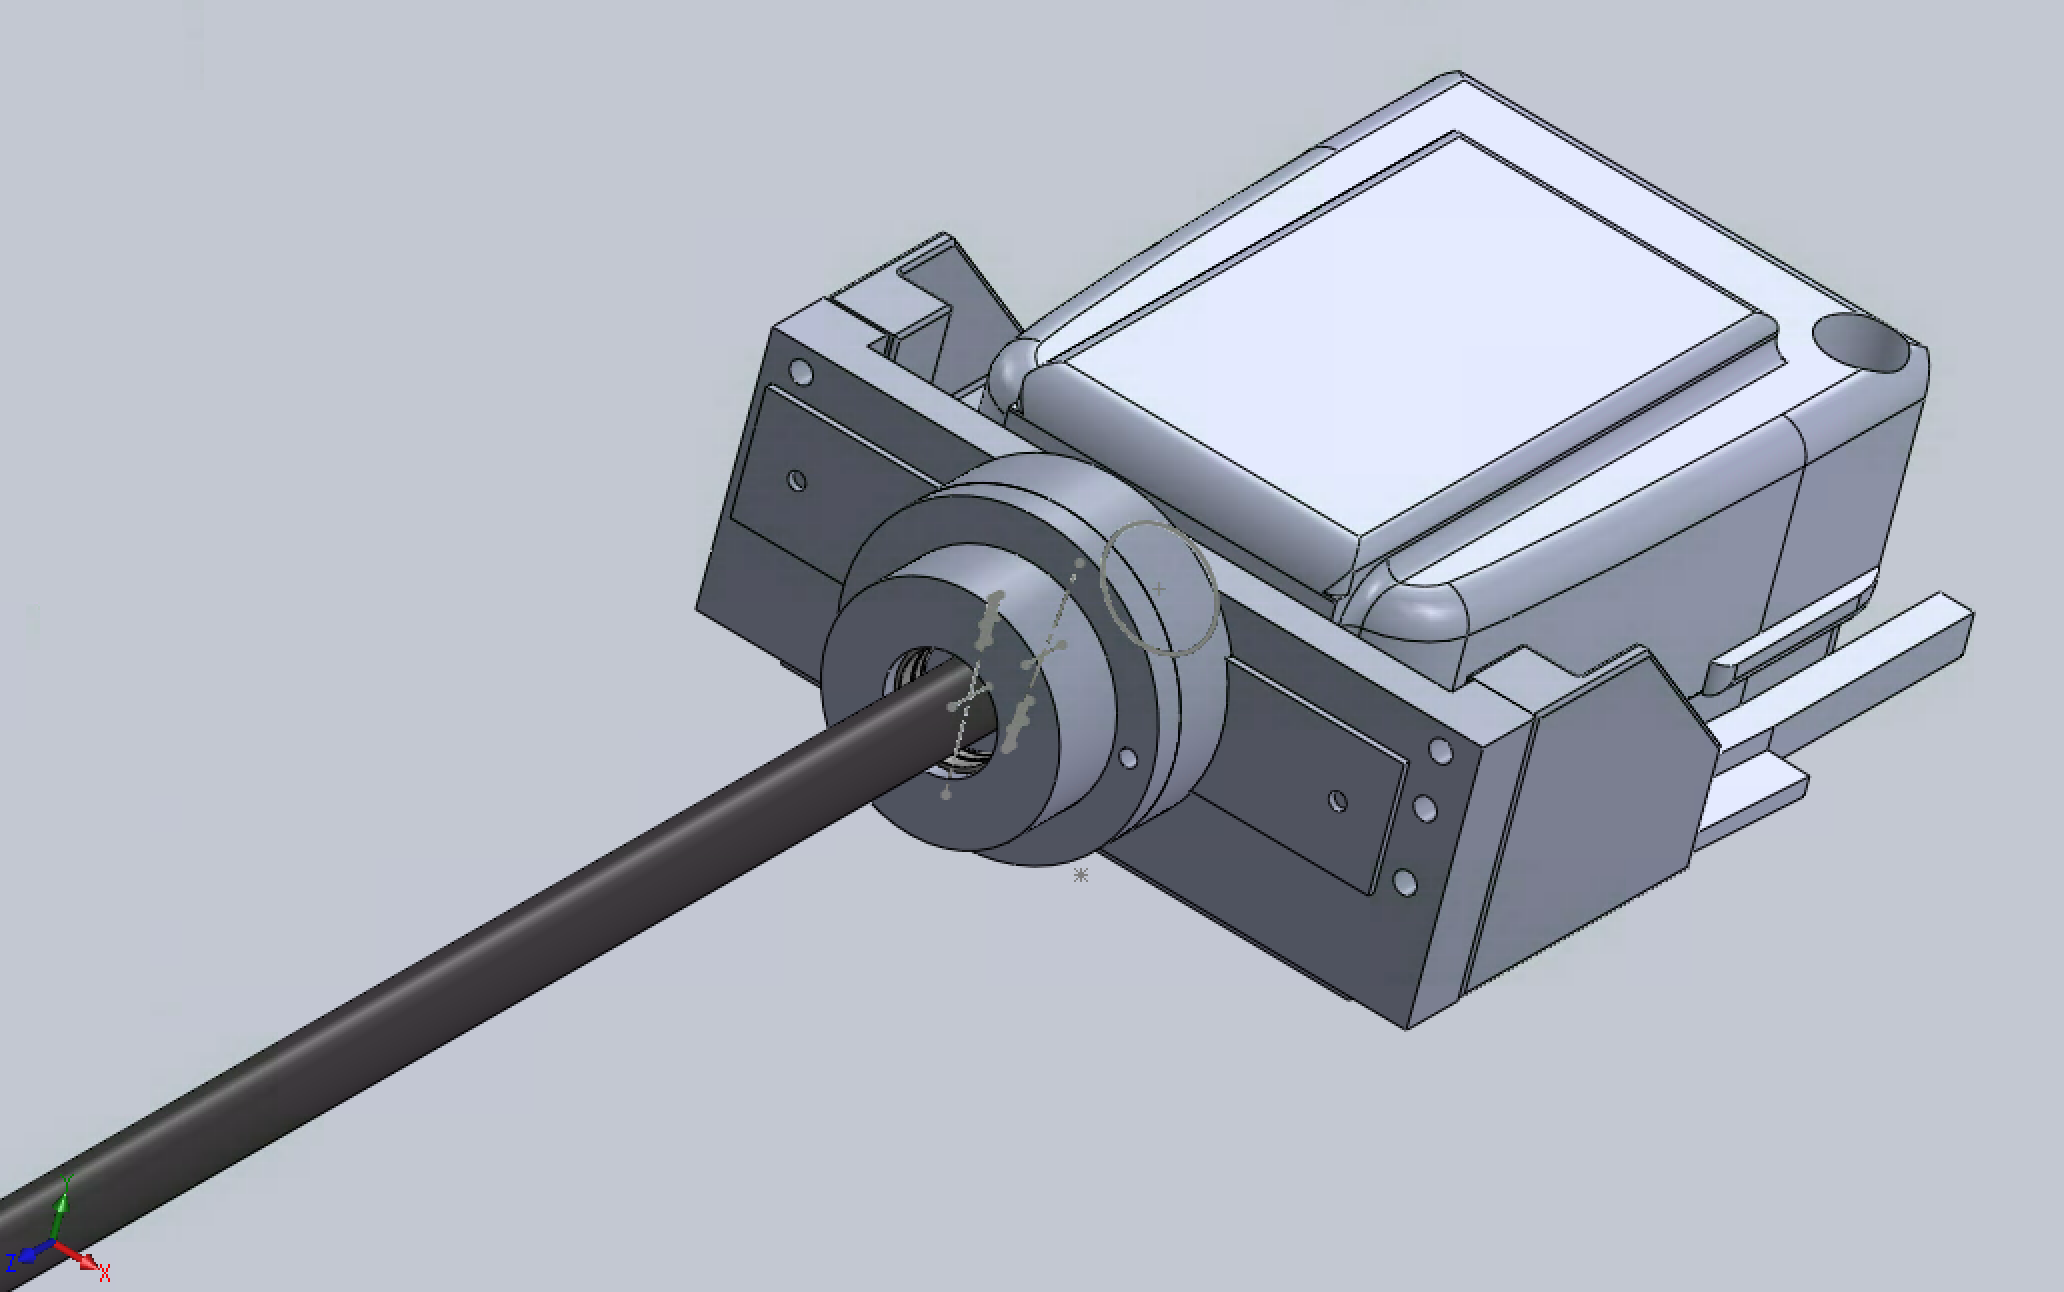
\includegraphics[width=120mm]{fig/methods/z_dir.png}
			\end{center}
			\vspace{-4mm}
		\caption[Z-direction force feedback sensor]
		{Z-direction force feedback sensor}
		\label{fig:Z-direction}
		\vspace{-2mm}
		\end{figure}

		\begin{figure}
			\begin{center}
			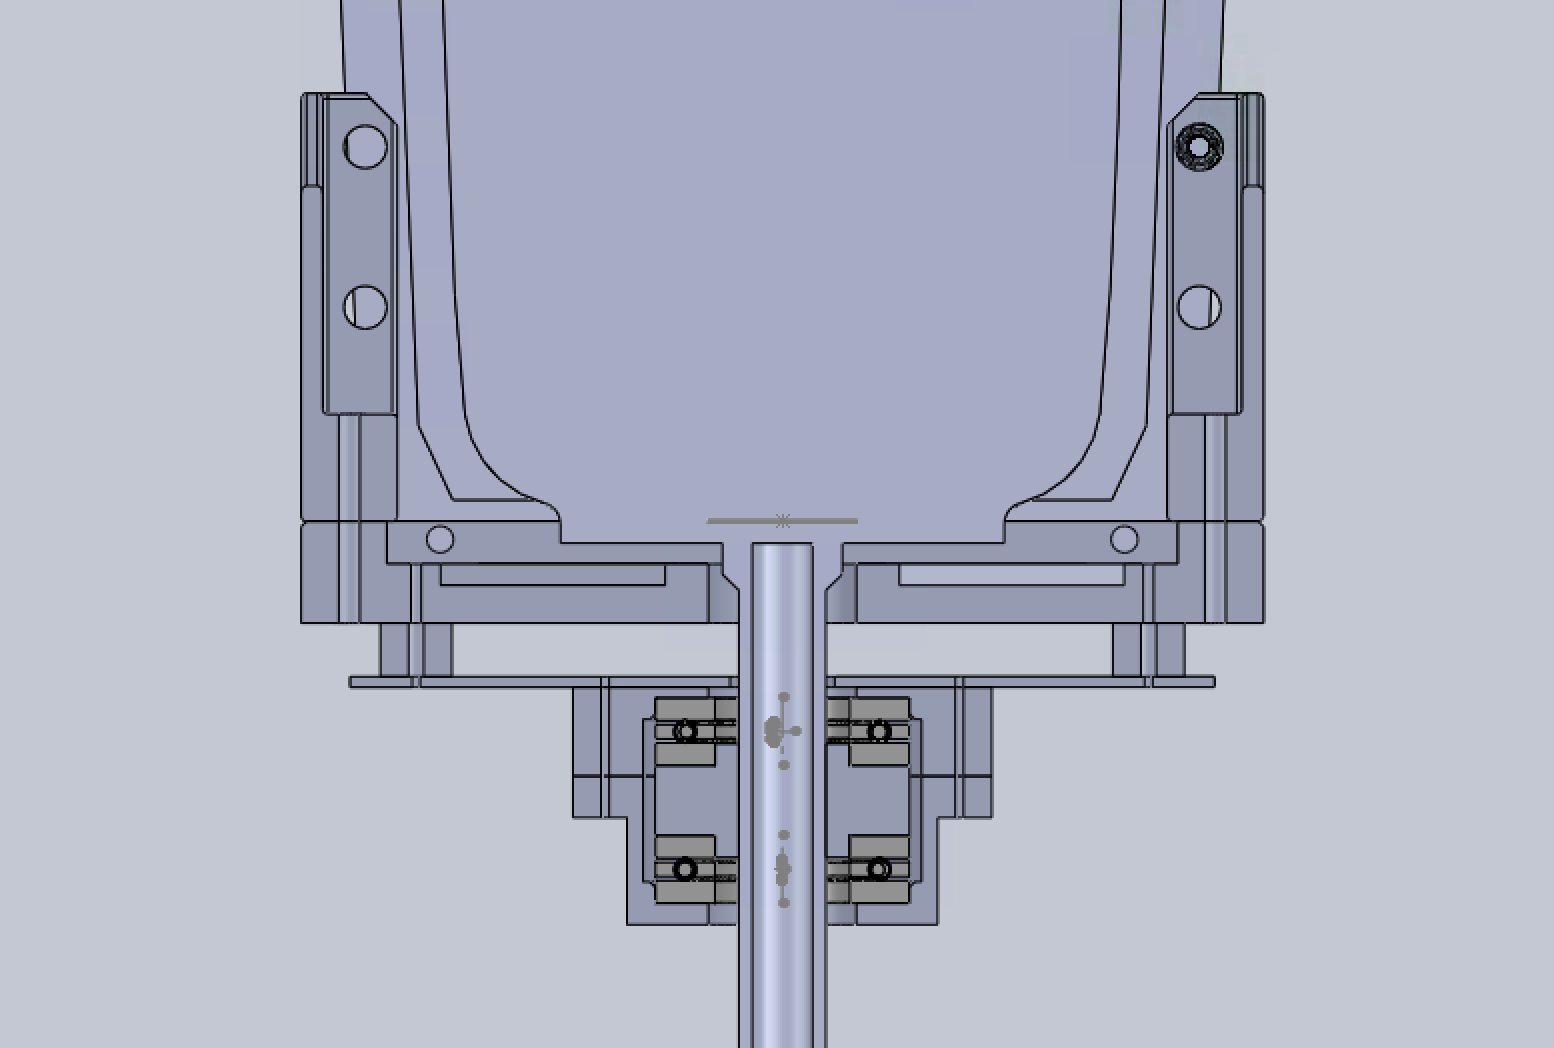
\includegraphics[width=120mm]{fig/methods/z_dir_sec.png}
			\end{center}
			\vspace{-4mm}
		\caption[Z-direction force feedback sensor - section vew]
		{Z-direction force feedback sensor - section vew}
		\label{fig:Z-direction_sec}
		\vspace{-2mm}
		\end{figure}

\section{Electrical and Software Design}
\label{sec:elecDes}

Using Altium Designer 15.1 PCB was developed and manufactured elsewhere. 

Write about how to calibrate the PCB itself and how it works.

	\subsection{Circuit design}
	\label{sec:cirDes}
	Write about how circuit works.

	\subsection{Noise Analysis}
	\label{sec:NoiseExp}
	Noise analysis was performed using oscilloscope ... Make FFT analysis

		\begin{figure}[h]
			\begin{center}
			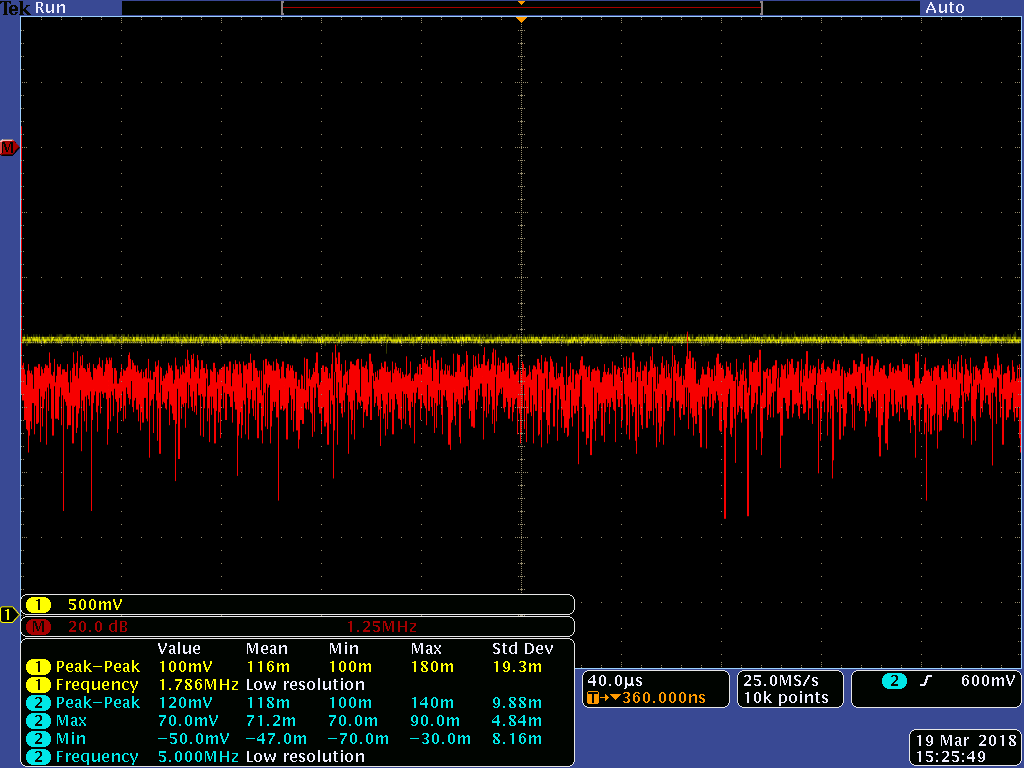
\includegraphics[width=120mm]{fig/results/40us_1stADC.png}
			\end{center}
			\vspace{-4mm}
		\caption[Noise analysis of the output signal]
		{Noise analysis of the output signal}
		\label{fig:OutputSignal}
		\vspace{-2mm}
		\end{figure}

	\subsection{Microcontroller Software}
	\label{sec:MicrSoft}
	We use arduino for ..
	Filtering was implemented on microcontroller by finding average of recent 5 readings 
	Filtering - ideally small time delay. Total teleoperation cycle delay - less than 100ms (visually noticeable delay). Kalman filter? Use same parameters for both signals to get identical time delay.
	good article about changing baud rate.

	\subsection{ROS Architecture}
	\label{sec:p2}
	
\section{Calibration}
\label{section:Calibration}
First we used set of weights applied in two directions, but since the system was too sensitive for direction of force, we had to change our approach of determining the force direction. It was decided to use optical tracking system for that purpose.

	\subsection{Calibration Setup}
	\label{sec:CalSetup}
	Tell how calibration with optical tracking system is working

	\subsection{Calibration of the Load Cell}
	\label{sec:CalLoadCell}
	Was pefrormed using following setup cite figure ..
	Calibration equation we got ..

	\subsection{Calibration Results}
	Find mean square root error

		\begin{figure}
			\centering
			\begin{subfigure}
				\centering
				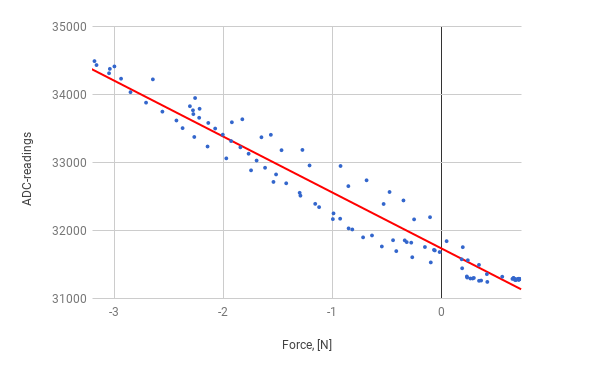
\includegraphics[width=120mm]{fig/results/x-dir.png}
				\caption{X-component}
				\label{fig:Xdirection}
			\end{subfigure}
			\begin{subfigure}
				\centering
				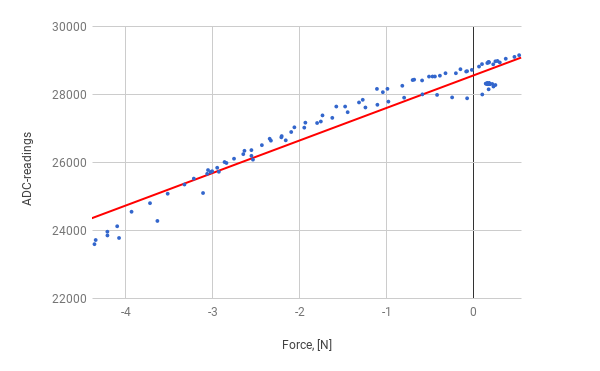
\includegraphics[width=120mm]{fig/results/y-dir.png}
				\caption{Y-component}
				\label{fig:Ydirection}
			\end{subfigure}
			\caption{Calibration results}
			\label{fig:Calibration}
		\end{figure}

\section{Experiments}
\label{sec:Experims}

	\subsection{Distance from the cannula to the tip dependence from readings}
	\label{sec:DisExp}
	Distance from the cannula to the tip - measure - 3 ¼ inch. Maximum distance is 9 inches.


	\subsection{Temeperature Dependence}
	\label{sec:TempExp}
	Try in 36.6 Celsius and room temperature
	Effect of the surrounding temperature on the device was ..

	Do all experiments at least three times and calculate all statistic things you can (SD)

	\subsection{Hysteresis}
	\label{sec:HystExp}
	Hysteresis was checked .. 
	We written separate program to check hysteresis